\documentclass{sa}
\usepackage{array} %dla poziomego wyrownania (m) w tabeli
\usepackage{soul}
\usepackage{bm}

\newcommand{\ang}[1]{(ang. \emph{#1})}
\renewcommand{\vec}[1]{\ensuremath\boldsymbol{#1}}
\newcommand{\grad}{\ensuremath\nabla}
\let\avg\overline

\usetikzlibrary{datavisualization}
\usetikzlibrary{datavisualization.formats.functions}

\tikzset{
layer/.style={rectangle,draw},
io/.style={rounded rectangle,draw},
node distance=.5cm
}

\newcommand{\nnconn}[3]{\draw[->] (#1) -- (#2) node[midway,right] {#3};}

\usepackage{hyperref}
\graphicspath{{08_autoencoders/}}
\subtitle{Autoenkodery}
\begin{document}
\begin{frame}
\titlepage
\end{frame}
\begin{frame}{Idea}
	\centering
	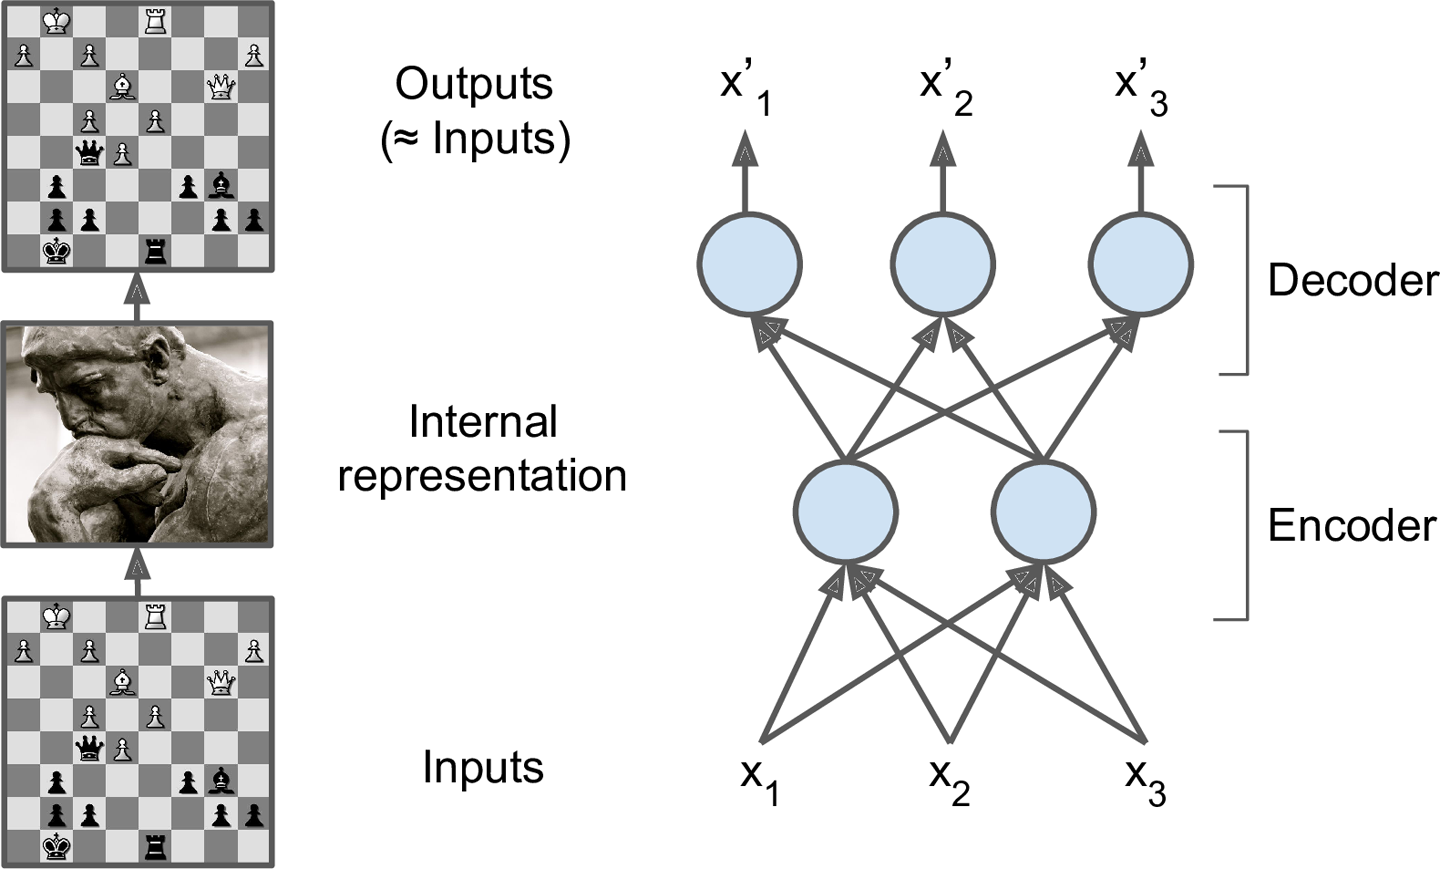
\includegraphics[width=\textwidth]{mlst_1501.png}
	{\vfill\footnotesize A. Géron, \emph{Hands-On Machine Learning with Scikit-Learn and TensorFlow} 2017}
\end{frame}
\begin{frame}{Lepsze i gorsze sposoby wyboru kodowania}
		\centering
	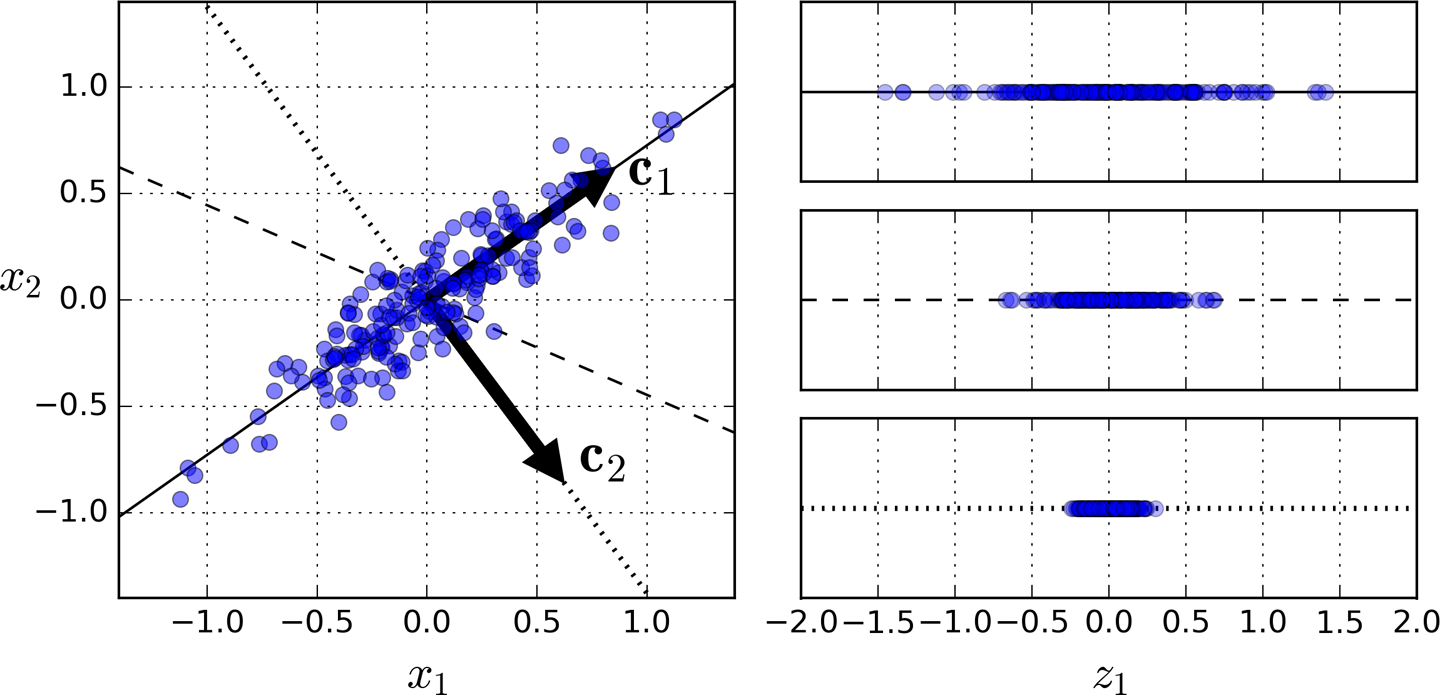
\includegraphics[width=\textwidth]{mlst_0807.png}
	{\vfill\footnotesize A. Géron, \emph{Hands-On Machine Learning with Scikit-Learn and TensorFlow} 2017}
\end{frame}
\begin{frame}{Rolada}
			\centering
	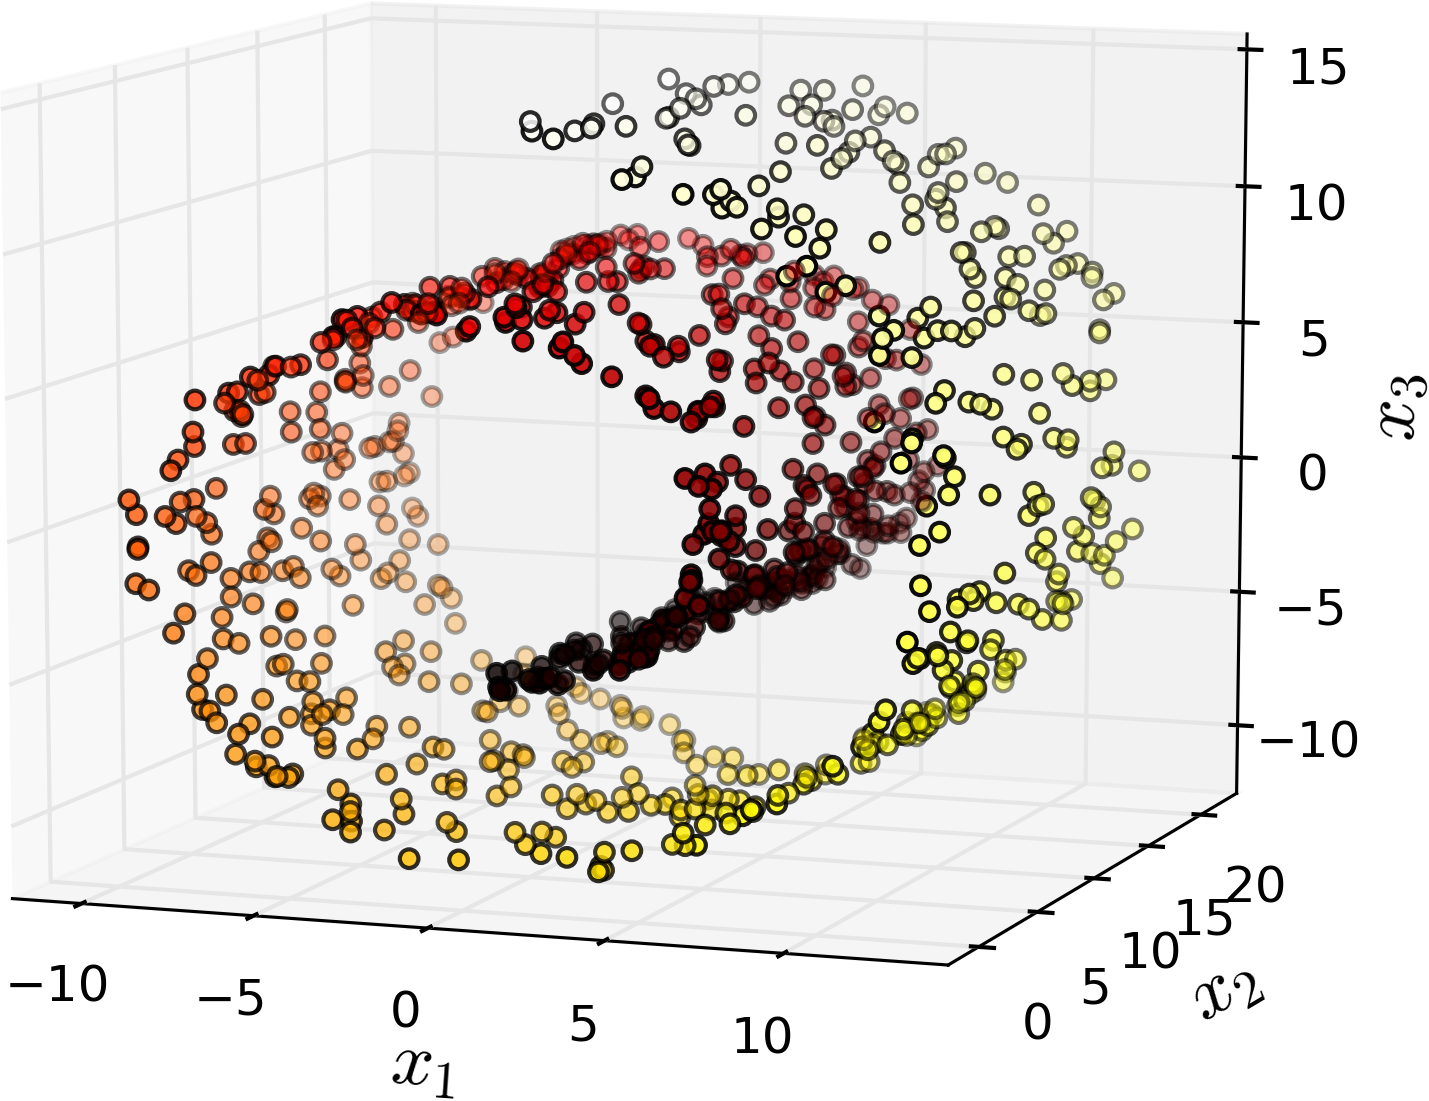
\includegraphics[width=.8\textwidth]{mlst_0804.png}
	{\vfill\footnotesize A. Géron, \emph{Hands-On Machine Learning with Scikit-Learn and TensorFlow} 2017}
\end{frame}
\begin{frame}{Spłaszczanie vs rozwijanie rolady}
	\centering
	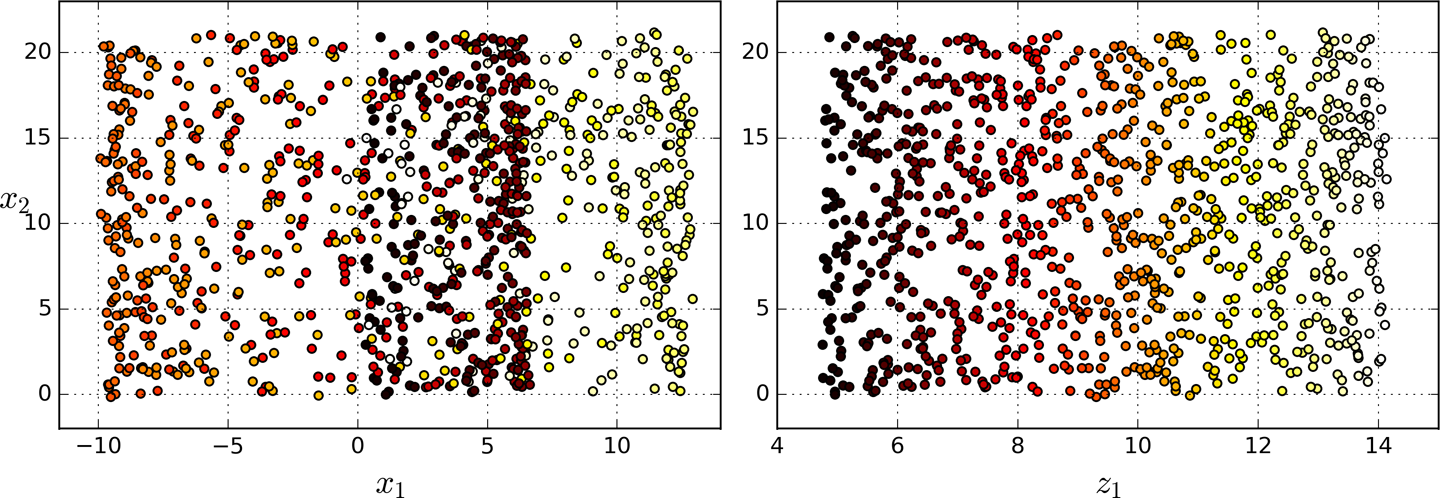
\includegraphics[width=\textwidth]{mlst_0805.png}
	{\vfill\footnotesize A. Géron, \emph{Hands-On Machine Learning with Scikit-Learn and TensorFlow} 2017}
\end{frame}
\begin{frame}{Głęboki autoencoder}
	\centering
	\begin{tikzpicture}
		\node [io] (input) {Wejście};
		\node [layer,minimum width=6cm,above=of input] (L1) {$L_1$};
		\node [layer,minimum width=3.5cm,above=of L1] (L2) {$L_2$};
		\node [io,minimum width=2cm,above=of L2] (code) {Kod};	
		\node [layer,minimum width=3.5cm,above=of code] (L3) {$L_3$ (zwykle: $L_3=L_2^T$)};
		\node [layer,minimum width=6cm,above=of L3] (L4) {$L_4$ (zwykle: $L_4=L_1^T$)};
		\node [io,above=of L4] (output) {Wyjście $\approx$ Wejście};
		\nnconn{input}{L1}{784};
		\nnconn{L1}{L2}{300};
		\nnconn{L2}{code}{150};
		\nnconn{code}{L3}{150};
		\nnconn{L3}{L4}{300};
		\nnconn{L4}{output}{784};	
	\end{tikzpicture}
	\note<1>
	{
		\begin{itemize}
			\item Liczby na krawedziach oznaczaja liczbe wartosci, czyli liczbe neuronow w warstwie, z ktorej wychodza. Oczywiscie sa to wartosci przykladowe.
			\item stosujemy zwyczajowe funkcje aktywacji
			\item funkcja celu: błąd średniokwadratowy między wejściem i wyjściem + regularyzacja
		\end{itemize}
	}
\end{frame}
\begin{frame}{Przykład}
	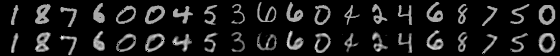
\includegraphics[width=\textwidth]{08_autoencoders/traditional.png}
	
	Jeden wiersz to przypadki testowe, a drugi to ich rekonstrukcje. Który jest który?
	
	\pause
	\vfill
	Parametry: 300 neuronów w L1, 40 neuronów w L2, MSE, brak regularyzacji, 6000 epok, rozmiar \emph{batcha} 128
\end{frame}
\begin{frame}{Trenowanie}
	\centering
	\begin{tikzpicture}

	\node (base) {};
			
	
	\node [layer,minimum width=5cm,right=of base] (ph2_L1) {$L_1$ zamrożone};
	\node [io,below=of ph2_L1] (ph2_input) {Wejście};
	\node [layer,minimum width=3cm,above=of ph2_L1] (ph2_L2) {$L_2$};
	\node [io,minimum width=2cm,above=of ph2_L2] (ph2_code) {Kod};	
	\node [layer,minimum width=3cm,above=of ph2_code] (ph2_L3) {$L_3$ (zwykle: $L_3=L_2^T$)};
	\node [layer,minimum width=5cm,above=of ph2_L3] (ph2_L4) {$L_4$ zamrożone};
	\node [io,above=of ph2_L4] (ph2_output) {Wyjście $\approx$ Wejście};
	\nnconn{ph2_input}{ph2_L1}{784};
	\nnconn{ph2_L1}{ph2_L2}{300};
	\nnconn{ph2_L2}{ph2_code}{150};
	\nnconn{ph2_code}{ph2_L3}{150};
	\nnconn{ph2_L3}{ph2_L4}{300};
	\nnconn{ph2_L4}{ph2_output}{784};

	\node [layer,minimum width=5cm,left=of base] (ph1_L1) {$L_1$};
	\node [io] (ph1_input) at (ph1_L1 |- ph2_input) {Wejście};
	\node  at (ph1_L1 |- ph2_L2) (ph1_L2) {};
	\node [io,minimum width=2cm] at (ph1_L1 |- ph2_code) (ph1_code) {Kod};	
	\node  at (ph1_L1 |- ph2_L3) (ph1_L3) {};
	\node [layer,minimum width=5cm]  at (ph1_L1 |- ph2_L4) (ph1_L4) {$L_4$ (zwykle: $L_4=L_1^T$)};
	\node [io]  at (ph1_L1 |- ph2_output) (ph1_output) {Wyjście $\approx$ Wejście};
	
	\nnconn{ph1_input}{ph1_L1}{784};
	\nnconn{ph1_L1}{ph1_code}{300};
	\nnconn{ph1_code}{ph1_L4}{300};
	\nnconn{ph1_L4}{ph1_output}{784};

	\draw[dashed] (base |- ph1_input) -- (base |- ph1_output);
	\end{tikzpicture}
	
\end{frame}
\begin{frame}{Wykorzystanie w uczeniu nadzorowanym}
	\begin{tikzpicture}
	
	\node (base) {};
	
	
	\node [layer,minimum width=5cm,left=of base] (ph1_L1) {$L_1$};
	\node [io,below=of ph1_L1] (ph1_input) {Wejście};
	\node [layer,minimum width=3cm,above=of ph1_L1] (ph1_L2) {$L_2$};
	\node [io,minimum width=2cm,above=of ph1_L2] (ph1_code) {Kod};	
	\node [layer,minimum width=3cm,above=of ph1_code] (ph1_L3) {$L_2^T$};
	\node [layer,minimum width=5cm,above=of ph1_L3] (ph1_L4) {$L_1^T$};
	\node [io,above=of ph1_L4]  (ph1_output) {Wyjście $\approx$ Wejście};
	
	\nnconn{ph1_input}{ph1_L1}{784};
	\nnconn{ph1_L1}{ph1_L2}{300};
	\nnconn{ph1_L2}{ph1_code}{150};
	\nnconn{ph1_code}{ph1_L3}{150};
	\nnconn{ph1_L3}{ph1_L4}{300};
	\nnconn{ph1_L4}{ph1_output}{784};
	
	\node [layer,minimum width=5cm,right=of base] (ph2_L1) {$L_1$ zamrożone};
	\node [io] at (ph2_L1 |- ph1_input) (ph2_input) {Wejście};
	\node [layer,minimum width=3cm] at (ph2_L1 |- ph1_L2) (ph2_L2) {$L_2$ zamrożone};
	\node [io,minimum width=2cm] at (ph2_L1 |- ph1_code) (ph2_code) {Kod};	
	\node [layer,minimum width=3cm] at (ph2_L1 |- ph1_L3) (ph2_L3) {$L_3$};
	%\node [layer,minimum width=5cm,above=of ph2_L3] (ph2_L4) {$L_4$ zamrożone};
	\node [io] at (ph2_L1 |- ph1_output) (ph2_output) {Etykieta};
	\nnconn{ph2_input}{ph2_L1}{784};
	\nnconn{ph2_L1}{ph2_L2}{300};
	\nnconn{ph2_L2}{ph2_code}{150};
	\nnconn{ph2_code}{ph2_L3}{150};
	\nnconn{ph2_L3}{ph2_output}{1};
	
	
	\draw[dashed] (base |- ph1_input) -- (base |- ph1_output);
	\end{tikzpicture}
\end{frame}
\begin{frame}{Autoenkodery usuwające szum}
		\centering
	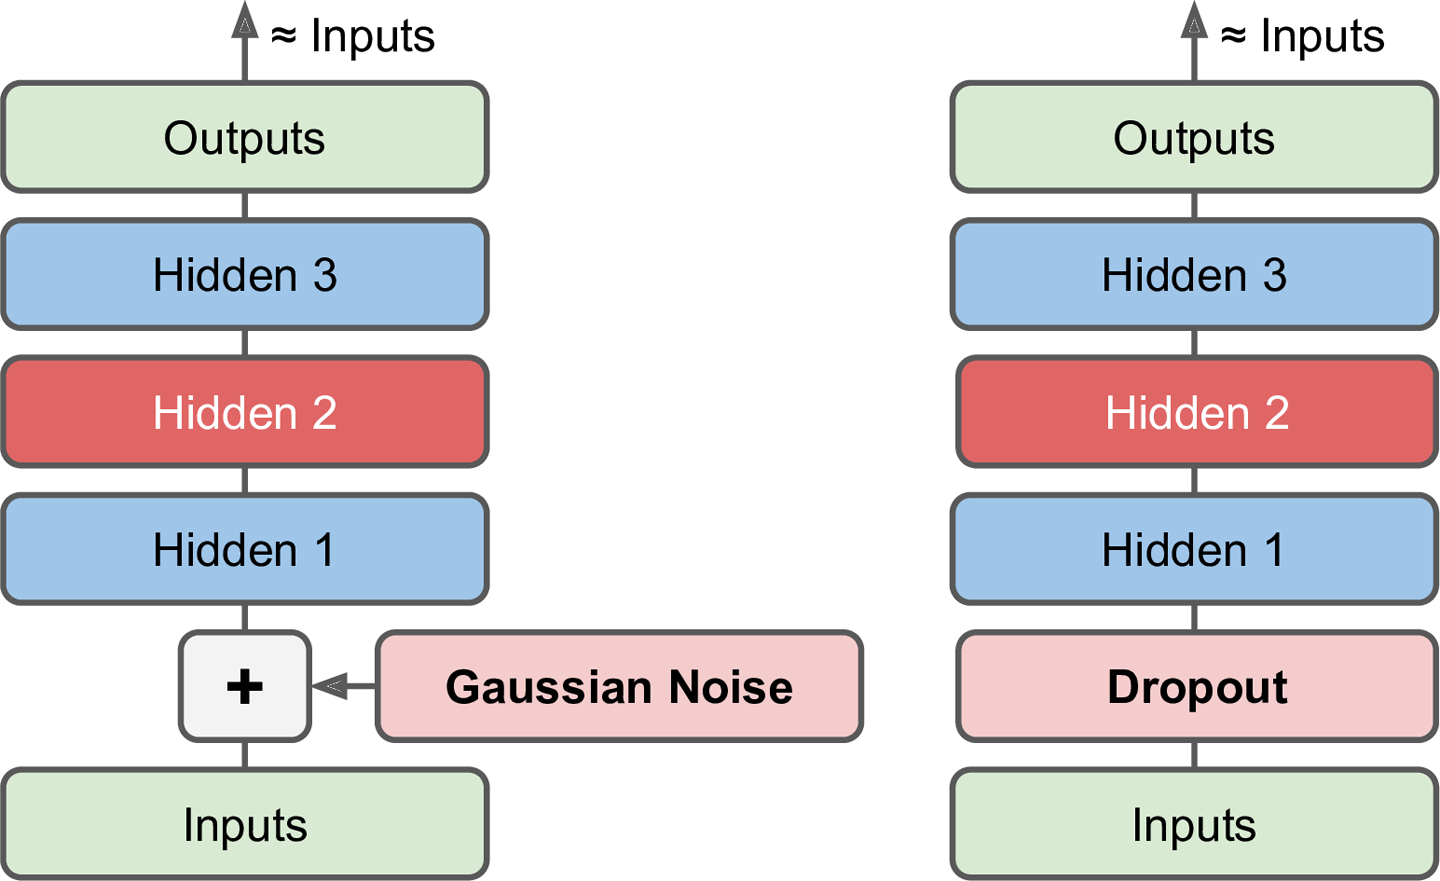
\includegraphics[width=\textwidth]{mlst_1509.png}
	{\vfill\footnotesize A. Géron, \emph{Hands-On Machine Learning with Scikit-Learn and TensorFlow} 2017}
\end{frame}
\begin{frame}{Autoenkodery wariacyjne (VAE -- variational autoencoder)}
	\begin{tikzpicture}
	\node [io] (input) {Wejście};
	\node [layer,minimum width=5cm,above=of input] (encoder) {Koder};
	\node [io,minimum width=2cm,above=of encoder] (mu) {$\boldsymbol{\mu}$};	
	\node [io,minimum width=2cm,right=of mu] (sigma) {$\boldsymbol{\sigma}$};	
	\node [layer,above=of mu] (sample) {próbka z $N(\boldsymbol{\mu}, \boldsymbol{\sigma})$};
	\node [io,minimum width=2cm,above=of sample] (code) {Kod};
	\node [layer,minimum width=5cm,above=of code] (decoder) {Dekoder};
	\node [io,above=of decoder] (output) {Wyjście $\approx$ Wejście};
	\nnconn{input}{encoder}{784};
	\nnconn{encoder}{mu}{2};
	\nnconn{encoder}{sigma}{2};
	\nnconn{mu}{sample}{2};
	\nnconn{sigma}{sample}{2};
	\nnconn{sample}{code}{2};
	\nnconn{code}{decoder}{2};
	\nnconn{decoder}{output}{784};	
	\end{tikzpicture}
\end{frame}
\begin{frame}{Problemy}
	\begin{itemize}
		\item $N(\boldsymbol{\mu}, \boldsymbol{\sigma})$ jest nieróżniczkowalne. Co z tym zrobić?
		\pause
		\item $\boldsymbol{\sigma}$ musi być dodatnie. Jak to zapewnić?
		\pause
		\item Czy sama kara za rekonstrukcję (np. MSE) wystarczy, żeby kod pochodził z wielowymiarowego rozkładu normalnego?
	\end{itemize}
\end{frame}
\begin{frame}{Regularyzacja}
	Chcielibyśmy, żeby rozkłady były jak najbardziej podobne do $N(0, 1)$. Dlaczego?\\
	\pause
	Czy wystarczy policzyć MSE pomiędzy $\boldsymbol{\mu}$, a $0$ oraz MSE pomiędzy $\boldsymbol{\sigma}$, a $1$?
	\pause
	Dywergencja Kullbacka–Leiblera
	\[ D_{KL}(P || Q) = \int_{-\infty}^\infty p(x) \log \frac{p(x)}{q(x)} \, dx \]
	\pause
	Dla $p(x)=N(\boldsymbol{\mu}, \text{diag}(\boldsymbol{\sigma}))$ i $q(x)=N(0,1)$:
	\[ D_{KL}(P || Q) = \frac{1}{2}\sum_{i=1}^n \left(  \mu_i^2 + \sigma_i^2 - \log \sigma_i^2 -1 \right) \]
	\note<1>{Jeżeli nie postawimy tego wymagania, to średnie mogą być dowolnie duże, odchylenia standardowe dowolnie małe, a zatem każda klasa obrazów może zająć własny kawałek przestrzeni kodów, tak jak to ma miejsce w normalnym autoenkoderze.}
	\note<2>{MSE to za mało, bo nie każe wystarczająco mocno za zbyt małe odchylenie standardowe. Z kolei dodanie 1 do $\sigma$ powoduje, że nie można z odchyleniem standardowym zejść poniżej 1, co mimo wszystko może być pożądane.
	}
\end{frame}
\begin{frame}{Przykład: rekonstrukcja (dla bardzo małego kodu!)}
	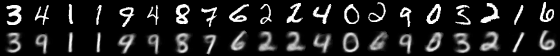
\includegraphics[width=\textwidth]{vae-rekonstrukcja.png}
\end{frame}
\begin{frame}{Przykład: generowanie ($\text{kod}\sim N(0,1)$)}
	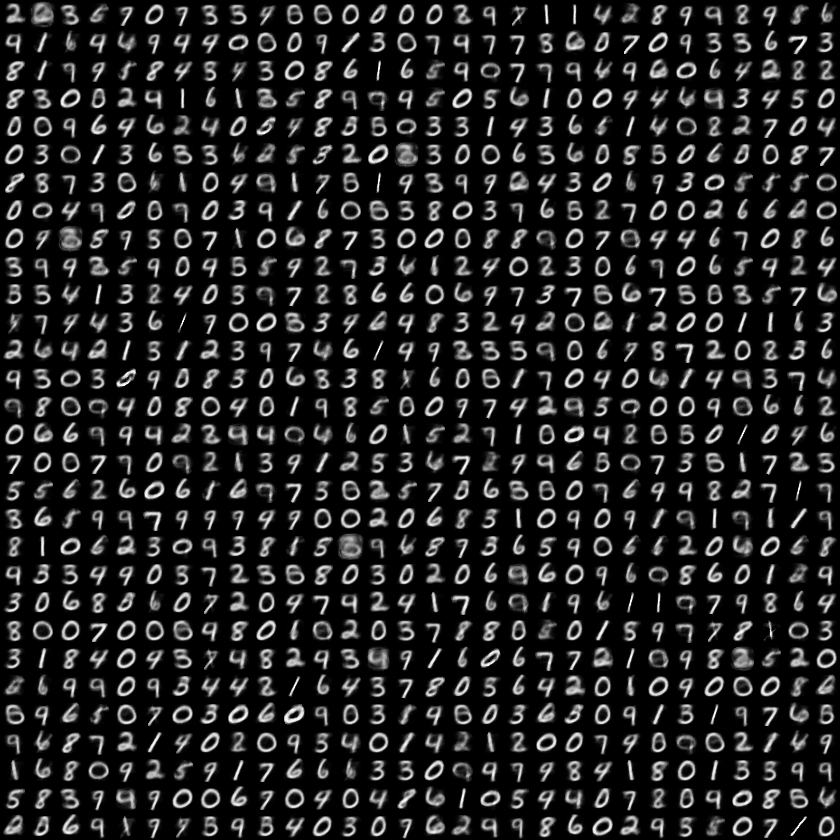
\includegraphics[width=\textwidth]{vae-generator.png}
\end{frame}
\begin{frame}{Przykład: wizualizacja przestrzeni kodów}
	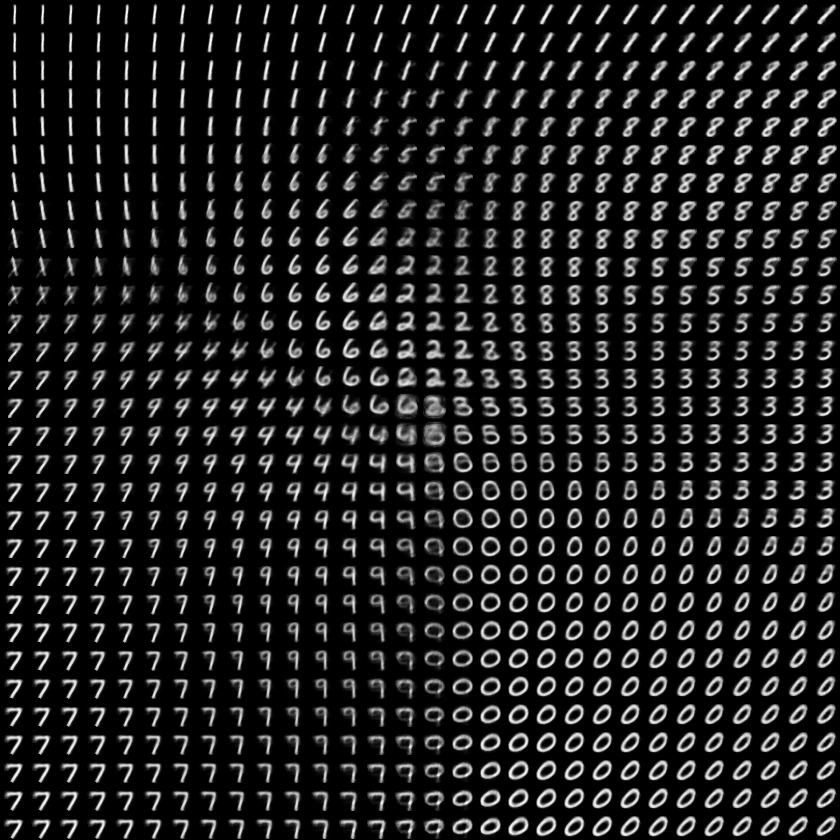
\includegraphics[width=\textwidth]{vae-latent.png}
	\note<1> {
		Dwuwymiarowy kod, na rysunku wartości od $-2$ do $2$, 30 równorozłożonych wartości w każdym z wymiarów.
	}
\end{frame}
%\begin{frame}{Funkcja kosztu w VAE}
%	\[
%		\frac{1}{2}\sum_{j=1}^J \left(1 + \log((\sigma_j)^2) - \mu_j^2 -\sigma_j^2\right)
%	\]
%\end{frame}
%%TODO funkcja kosztu
%%TODO GAN
\end{document}